\documentclass[12pt]{article}
\thispagestyle{empty}
\usepackage{amsmath}
\usepackage[margin=1in]{geometry}
\usepackage{amsfonts}
\usepackage{hyperref}
\usepackage{graphicx}
\usepackage{siunitx}
\usepackage{cancel}
\usepackage{xfrac}
\usepackage{listings}

\begin{document}

	\begin{center}
	\par\noindent \large \textbf{Binary Arithmetic (part 2)}  [ Andy Chong Sam ]
	\end{center}	
	\par\noindent {\textbf{1   Binary Multiplication} }
	\newline
	\newline
	\begin{minipage}[t]{.5\linewidth}
	\par\noindent \textbf{(I)} First, some foundational operations, with their decimal equivalents on the right:
	\begin{flalign*}
		\textbf{Binary} \;\;\;\;\;\; \textbf{Decimal} \\
		0 \times 0 = 0 \;\;\;\;\;\; 0 \times 0 = 0 \\
		1 \times 0 = 0 \;\;\;\;\;\;1 \times 0 =0 \\
		1 \times 1 = 1 \;\;\;\;\;\; 1 \times 1 = 1 \\
	\end{flalign*}
	\par\noindent \textbf{(II)} We carry out binary multiplication the same way we would with decimal numbers, by arranging our results in columns. Let's consider the case of \(2 \times 3 = 6\). In binary \(2\) is \(10\) and \(3\) is \(11\):

	\begin{center}
		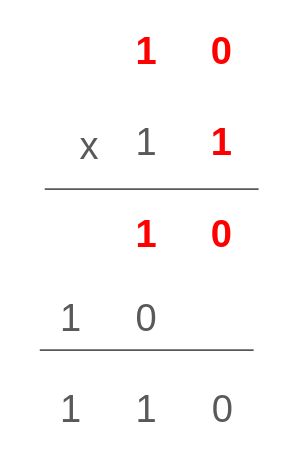
\includegraphics[width=2.5cm]{bin-multi-1.png}
	\end{center}

	\par\noindent We populate the first result column by carrying out \(1 \times 0 = 0\) followed by \(1 \times 1 =1\). This is show in red above.
	
	\begin{center}
		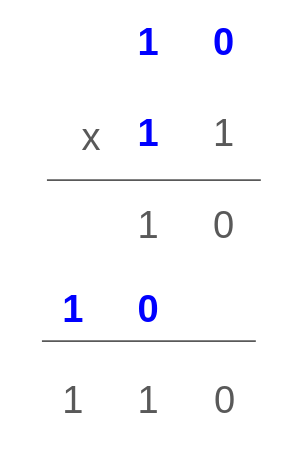
\includegraphics[width=2.5cm]{bin-multi-2.png}
	\end{center}

	\par\noindent We now multiply the digits in blue \(1 \times 0 = 0\) and \(1 \times 1 = 1\) and populate the second result column. We conclude by adding the columns to get \(110\) which is indeed the binary representation of 6.
	\end{minipage}
	\hspace{0.45cm}
	\begin{minipage}[t]{.5\linewidth} 
		
		\par\noindent \textbf{(III)} Now let's try a trickier operation, suppose we wanted to evaluate \(7 \times 7 = 49\) which in binary is \(111 \times 111\). When we finish the multiplication phase we are left with the following three rows:
		
		\begin{center}
		 	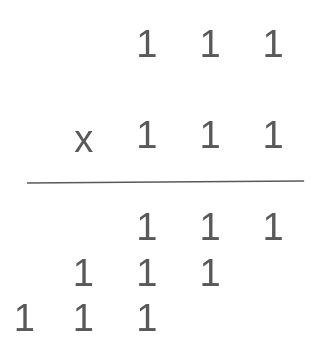
\includegraphics[width=2.7cm]{bin-multi-3.png}
		\end{center}
	
		\par\noindent After adding the first two columns we have:
		
		\begin{center}
			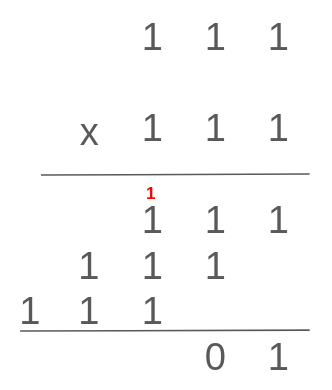
\includegraphics[width=3.0cm]{bin-multi-4.png}
		\end{center}
	
		\par\noindent On the third column, we are evaluating \(1 + 1 + 1 + 1 = 4\) which in binary is \(100\). We will record the right most zero, send the center zero to the next column's carry, and finally the one to the column after that. This result is shown below in blue:
		
		\begin{center}
			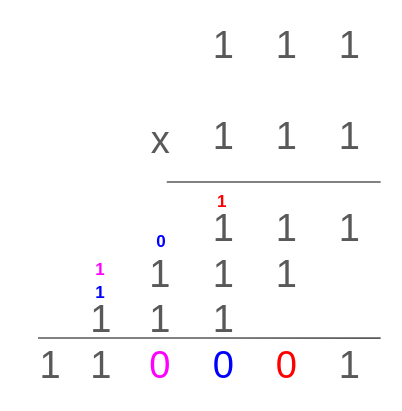
\includegraphics[width=4.0cm]{bin-multi-5.png}
		\end{center}
	
		\par\noindent Adding all the columns gets us \(110001\), the binary representation of 49.
		
	\end{minipage}
	\newpage
		\par\noindent {\textbf{2   Binary Division} }
	\newline
	\newline
	\begin{minipage}[t]{.5\linewidth}
		\par\noindent \textbf{(I)} As you might have guessed we can recycle another technique from decimal math. Binary division is best handled through long division. We will use the following terms: the dividend (the number we are dividing), divisor (what we are dividing by), the quotient, and the remainder.
		\newline
		\par\noindent \textbf{(II)} Let's consider the case of \(4 \div 2 = 2\). The number 4 in binary is \(100\) and 2 is \(10\), so we have:
		
		\begin{center}
			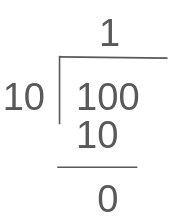
\includegraphics[width=2.0cm]{bin-div-1.png}
		\end{center}
	
		\par\noindent On the calculation above, the first step is shown, the \(10\) in the divisor goes evenly into the first two digits of the dividend producing a remainder of 0. We pull down the next digit in the dividend:
		
		\begin{center}
			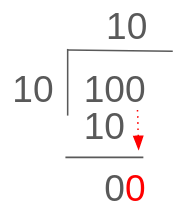
\includegraphics[width=2.0cm]{bin-div-2.png}
		\end{center}
	
		\par\noindent Since \(00\) is less than \(10\) we place a 0 on the quotient next to the one. Lastly \(10\) can go 0 times into \(00\) so documenting this gets us a quotient of 10, the binary representation of 2:
		
		\begin{center}
			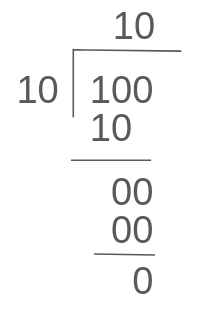
\includegraphics[width=2.0cm]{bin-div-6.png}
		\end{center}
	
	\end{minipage}
	\hspace{0.45cm}
	\begin{minipage}[t]{.5\linewidth} 
		\par\noindent \textbf{(III)} Now let's try the operation \(15 \div 2\), which will result in a quotient of 7 and a remainder of 1. In binary, 15 is \(1111\). Here is the first step:
		
		\begin{center}
			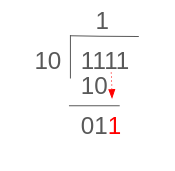
\includegraphics[width=2.7cm]{bin-div-3.png}
		\end{center}
	
		\par\noindent In the next step, after the 1 is pulled down, we can fit \(10\) into \(11\) but with a remainder of 1 (this operation is the subtraction \(011-010\)):	
		
		\begin{center}
			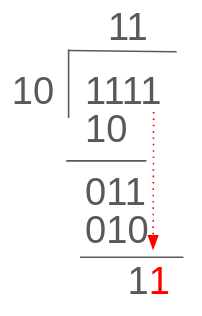
\includegraphics[width=2.0cm]{bin-div-4.png}
		\end{center}
		
		\par\noindent After again pulling down the next digit, which happens to be a 1, we can fit the \(10\) into \(11\) with a remainder of 1:
		
				\begin{center}
			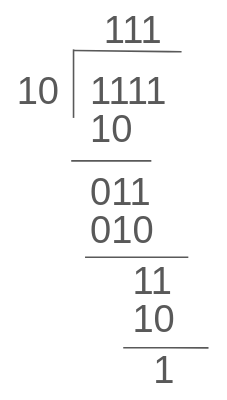
\includegraphics[width=2.2cm]{bin-div-5.png}
		\end{center}
	
		\par\noindent There are no more digits to pull down so we are done. Upon completing the final subtraction we find that the result is a quotient of \(111\) (binary for 7) and a remainder of 1.
	
	\end{minipage}
\end{document}